\documentclass{article}

\usepackage{graphicx}
\usepackage{longtable}
\usepackage{subcaption}
\usepackage{caption}
\usepackage{float}
\usepackage{comment}
\graphicspath{{./Images/}}

\begin{document}

\begin{figure}
\centering
	
\includegraphics[height=8cm]{Images/polimi_logo}
\end{figure}
	
\title {{\Huge \it SafeStreets} \\ \Large Software Engineering 2 Project - Prof. Matteo Rossi \\ {\bf DD Document}}
\author{Salvatore Fadda - 944786\\Adriano Mundo - 944684 \\ Francesco Rota - 948714
		\\ \\ A.Y. 2019/2020 \\ Version 1.0}
\date{December 9, 2019}	

\maketitle
\newpage

% Index	
\tableofcontents
\newpage

% Introduction - Section 1
\section{Introduction}
	\subsection{Purpose}
	This document represent the {\it Design Document} (DD). It aims at providing an in-depth description of the architecture below {\it SafeStreets} application and its services. It will present a section related to the architectural design with different perspective on the components of the {\it System}, how they interact and how they will be implemented. All the requirements of the RASD document are mapped with the components to explain how they will be satisfied. Finally, a section for the testing plan for Q\&A team is provided.
		
	\subsection{Scope}
	{\it SafeStreets} is a crowd-sourced application that aims at keeping safe the city's streets. The idea behind this service is to allow {\it Users} to notify the {\it Municipality} when a violation occur on the streets under its jurisdiction. The {\it User} can notice and notify the violation by sending a photo of the violation including date, time and position. {\it SafesStreets} stores all the data and uses a plate recognition algorithm to recognise the image content. \\ \\
	The {\bf Basic Service} allows {\it Users} and {\it Authorities} to mine the information \mbox{collected} by the service, so they can access statistics built from the data. \\ \\
	As {\bf AF1}, the application {\it SafeStreets} identifies potentially unsafe areas and \mbox{suggests} possible interventions to {\it Authorities} to solve the founded issues. \\ \\ 
	As {\bf AF2}. the application {\it SafeStreets} allows the {\it Municipality} to generate \mbox{traffic} tickets directly from the application data. Also, using the data of issued tickets the {\it System} can build statistics and find insights to suggest to {\it Municipality} in order to improve their service.
		
	\subsection{Definitions, Acronyms, Abbreviations}
		\subsubsection{Definitions}
			\begin{itemize}
				\item {\bf Client:} a piece of computer hardware or software that accesses a service made available by a Server. 
				\item {\bf Server:} a computer program or a device that provides functionality and handle the requests of other programs or devices, called Clients. 
				\item {\bf N-Tier:} or multilayer is an architecture in which presentation, application processing, and data management functions are physically separated in n-layers. 
				%%\item {\bf Design Pattern:}
				%%\item {\bf Proxy:}
			\end{itemize}
	
	
		\subsubsection{Acronyms}
			\begin{itemize}
				\item {\bf GPS:} Global Positioning System
				\item {\bf API:} Application Programming Interface
				\item {\bf RASD:} Requirements Analysis and Specification Document
				\item {\bf DBMS:} Data Bases Management System
				\item {\bf GDPR:} General Data Protection Regulation
				\item {\bf MVC:} Model-View-Controller
				\item {\bf REST:} REpresentational State Transfer
				\item {\bf Q\&A:} Quality and Assurance
				\item {\bf UI:} User Interface
				\item {\bf HTTPS:} Hyper Text Transfer Protocol Secure
			\end{itemize}
		
		\subsubsection{Abbreviations}
			\begin{itemize}
				\item {\bf [Rn]:} n-th Functional Requirement
				\item {\bf A1:} Advanced Function One
				\item {\bf A2:} Advanced Function Two 
			\end{itemize}
	
	
		\subsection{Revision history}
			\begin{table}[ht]
				\centering
				\begin{tabular}{ccc} 
				Version & Date & Description  \\ 
				\hline
		 		\\1.0 & 09/12/2019 & First Delivery
		 		\\
			\end{tabular}
			\caption{Revision History}
			\label{default}
		\end{table}
	
	
		\subsection{Reference Documents}
			\begin{itemize}
				\item Mandatory Project Assignment
				\item RASD Document of {\it SafeStreets} application
			\end{itemize} 
	
		\subsection{Document Structure}
		The other sections of the Design Document (DD) are organised in this way:
			\begin{itemize}
				\item {\bf Architectural Design} (Section 2): an in-depth description of the System's architecture. It defines the main components, the relationship between them and the deployment of components. There are different views and levels of analysis of the components plus some subsection useful for identifying how the components interact and the architectural styles and patterns. 
				\item {\bf User Interface Design} (Section 3): a complementary section of what was included in the RASD. It includes the definition of the UX process through a model that represents the flows of the interfaces. 
				\item {\bf Requirements Traceability} (Section 4): a complementary section of what was included in the RASD. It contains all the identified requirements and show the relationship between them and design choices in order to satisfy them. 
				\item {\bf Implementation, Integration and Test Plan} (Section 5): shows the order of the implementation and integration of all the components and subcomponents, providing how the application will be tested.
				\item {\bf Effort Spent} (Section 6): a section containing a table for identifying the hours and the effort spent by each team member to deliver the DD.
			\end{itemize}
		
		\pagebreak
	
	
% Architectural Design - Section 2
\section{Architectural Design}
	\subsection{Overview}
		\begin{figure}[H]
			\centering
			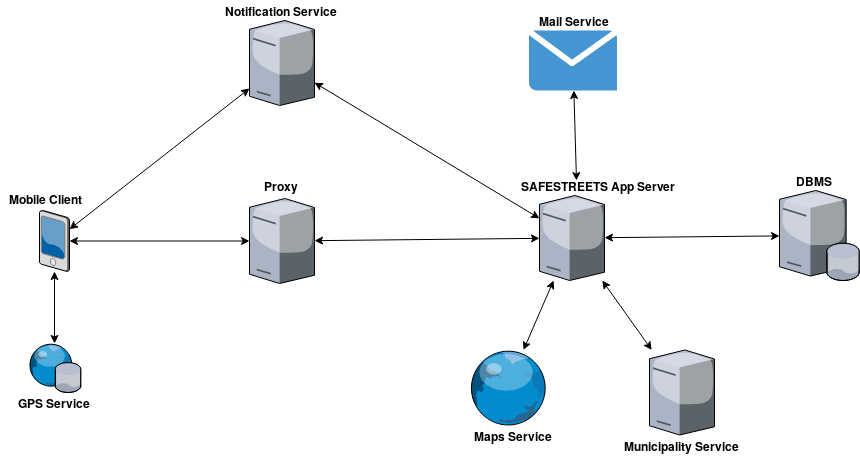
\includegraphics[scale=0.5]{Images/Overview.png}
			\caption{{\it SafeStreets} Overview of the System}
		\end{figure}
	The image above shows an high-level overview of the {\it System}'s architecture.
	The components interact with some external services. \\
	The Mobile Client application accesses the GPS service in order to retrive geographical information and communicates with the Application Server through a Proxy. \\ The Application Server uses an external Notification Service to send notifications directly to the Client. It uses a Mail System service and a Map service to execute all the functions. Finally, it accesses the Municipality Service to retrieve data and to communicate with the Municipality through the an API service offered by the Municipality itself.\\ 
	Further details on the {\it System} components will be explained in the next sections. 		
	
		
	\subsection{Component view}
	
		
	\subsection{Deployment view}
	
		
	\subsection{Runtime view}
	
	
	\subsection{Selected architectural styles and patterns}
	
	
	\subsection{Other design decisions}
	

% User Interface Design - Section 3
\section{User Interface Design}

% Requirements Traceability
\section{Requirements Traceability}
	
	\begin{longtable}{| p{5 cm} | p{8 cm} |} \hline
		Component (DD) & Requirements (RASD)  \\ \hline
		\newline Component Name & 
		\begin{itemize}
			\item 
		\end{itemize}	\\ \hline
		\newline Component Name 2 & 
		\begin{itemize}
			\item  
		\end{itemize}		\\	 \hline				
		\caption{Requirements Traceability}	
		
	\end{longtable}
	
	
% Testing - Section 5
\section{Implementation, Integration and Test Plan}
	\subsection{Overview}
		
	\subsection{Implementation}
	
		
% Effort - Section 6
\section{Effort Spent}
	
	
\end{document}
